%%%%%%%%%%%%%%%%%%%%%%%%%%%%%%%%%%%%%%%%%%%%%%%%%%%%%%%%
%%%%%%%%%------NAPB2019 adopted based on RMIT SPACE POSTER------------%%%%%%%%%%%%
%%%%%%%%%%%%%%%%%%%%%%%%%%%%%%%%%%%%%%%%%%%%%%%%%%%%%%%%
%%%%%%%%%%%%%%%%%%%%%%%%%%%%%%%%%%%%%%%%%%%%%%%%%%%%%%%%
% a0poster Portrait Poster
%
% The a0poster class was created by:
% Gerlinde Kettl and Matthias Weiser (tex@kettl.de)
% 
% License:
% CC BY-NC-SA 3.0 (http://creativecommons.org/licenses/by-nc-sa/3.0/)
%
% Author/Designer: Sirjan Sapkota
% Original Design by : Timothy Kodikara (RMIT Space Poster)
%
%% Note: CRC and SERC logos are included in the /figures folder if you might want to use them.
%%%%%%%%%%%%%%%%%%%%%%%%%%%%%%%%%%%%%%%%%
%----------------------------------------------------------------------------------------
%	PACKAGES AND OTHER DOCUMENT CONFIGURATIONS
%----------------------------------------------------------------------------------------
\documentclass[a0,portrait]{a0poster}
%%
\usepackage[top=5cm, bottom=0.1cm, left=5cm, right=1cm]{geometry}
\usepackage[compact]{titlesec}
\usepackage{multicol} % This is so we can have multiple columns of text side-by-side
\columnsep=50pt % This is the amount of white space between the columns in the poster
\columnseprule=5pt % This is the thickness of the blue line between the columns in the poster
\usepackage[svgnames]{xcolor} % Specify colors by their 'svgnames', for a full list of all colors available see here: http://www.latextemplates.com/svgnames-colors
%\usepackage{times} % Use the times font
\usepackage{palatino} % Uncomment to use the Palatino font
\usepackage{xkeyval}
\usepackage{graphicx} % Required for including images
\usepackage{subcaption}
\setlength{\abovecaptionskip}{5pt plus 5pt minus 3pt}
\graphicspath{{figures/}} % Location of the graphics files
\usepackage{booktabs} % Top and bottom rules for table
\usepackage[font=small,labelfont=bf]{caption} % Required for specifying captions to tables and figures
\usepackage{amsfonts, amsmath, amsthm, amssymb} % For math fonts, symbols and environments
\usepackage{csquotes}
\usepackage{wrapfig} % Allows wrapping text around tables and figures
%\usepackage[pdftex]{color}
\def\columnseprulecolor{\color{Orange}}%
\usepackage{framed}
\colorlet{frameborder}{NavyBlue}
\usepackage{environ}
\NewEnviron{myequation}{%to make an separate environment for each equation
    \begin{equation}
    \scalebox{1.5}{$\BODY$}
    \end{equation}
    }

\fboxrule0pt

\definecolor{rahmen}{RGB}{0,73,114}
\definecolor{grund}{RGB}{238,241,251}          
\definecolor{schrift}{RGB}{0,73,114}
\definecolor{bananamania}{RGB}{0.98, 0.91, 0.71}
\definecolor{beige}{rgb}{0.96, 0.96, 0.86}
\definecolor{bluebell}{rgb}{0.64, 0.64, 0.82}
\definecolor{palechestnut}{rgb}{0.87, 0.68, 0.69}
\definecolor{pastelblue}{rgb}{0.68, 0.78, 0.81}
\definecolor{sikusa1}{rgb}{0.9, 0.9, 0.6}
\definecolor{peachpuff}{rgb}{1.0, 0.85, 0.73}
\definecolor{periwinkle}{rgb}{0.8, 0.8, 1.0}
\definecolor{aliceblue}{rgb}{0.94, 0.97, 1.0}
\definecolor{charcoal}{rgb}{0.21, 0.27, 0.31}
\definecolor{coolblack}{rgb}{0.0, 0.18, 0.39}


%----------------------------------------------------------------------------------------
%	POSTER HEADER 
%----------------------------------------------------------------------------------------
% The header is divided into three boxes:
% The widths of these boxes can be easily edited to accommodate your content as you see fit
\begin{document}

%\hspace*{0.5cm}
\begin{minipage}[c]{\linewidth}
\vspace{0.1cm}
\noindent\makebox[\textwidth][c]{
\begin{minipage}[c]{0.15\linewidth}
\vspace{0pt}\raggedright
\hspace{1cm}

\includegraphics[width=\linewidth]{Clemson_logo.png}
\end{minipage}
\hfill
\begin{minipage}[c]{0.70\textwidth}
\centering
\Huge \color{NavyBlue} \textbf{Impact of Racial Structure on Genomic Prediction for Grain Yield Components in Sorghum}\\[0.5cm]
\large \color{Black} \textbf{Sirjan Sapkota $^{1,2}$, Rick Boyles$^{1}$, Elizabeth Cooper$^{3}$, Zach Brenton$^{2}$, Matt Myers$^2$, and Stephen Kresovich $^{1,2}$}\\[0.2cm] % Author(s)
\small 1. Department of Plant and Environmental Sciences, Clemson University, Clemson SC, 29634\\[0.1cm] % University
\small 2. Advanced Plant Technology Program, Clemson University, Clemson SC, 29634\\[0.1cm] % Affiliation 2
\small 3. Department of Bioinformatics and Genomics, University of North Carolina at Charlotte, Charlotte, NC 28223\\[0.1cm]
\small \texttt{Correspondence: ssapkot@clemson.edu, GitHub: @sirjansapkota, @KresovichLab}\\
\end{minipage}
%\hfill
\begin{minipage}[c]{0.15\textwidth}
\vspace{0pt}\raggedleft

\includegraphics[scale=1,width=\linewidth]{pes-logo.png}
\hspace{1cm}
\end{minipage}}
\\[0.1cm]%
% A bit of extra whitespace between the header and poster content
%----------------------------------------------------------------------------------------
\color{Purple}\setlength\FrameRule{5pt}
\begin{framed}
\vspace{0.5cm}
\begin{multicols}{2} % This is how many columns your poster will be broken into, a portrait poster is generally split into 2 columns
%----------------------------------------------------------------------------------------
%	INTRODUCTION
%----------------------------------------------------------------------------------------
\color{Black}
\section*{BACKGROUND}
\textbf{SORGHUM} is an important cereal grain used for food, feed, and fuel. While the genetic gain in sorghum has not reached its genetic potential, the application of genomic tools could accelerate the exploitation of genetic diversity towards that goal. Breeding values of gene bank accessions can be estimated and novel germplasm with genetic potential can be incorporated into breeding gene pool, which consequently will enhance diversity and long term gain in breeding programs \citep{gorjanc2018optimal,yu2016genomic}.\\\\
\textbf{GENOMIC PREDICTION/SELECTION} (GP/GS) uses a trained prediction model to estimate marker effects and subsequently estimate breeding values of non-phenotyped germplasm using just the genetic markers (Fig. \ref{GS_pop}-left, \citep{Meuwissen1819}). In stratified populations, population structure have been shown to affect the accuracy of genomic prediction models \citep{guo2014impact}.\\
%\begin{wrapfigure}{R}{0.25\textwidth}
\begin{center}
\hspace*{\fill}
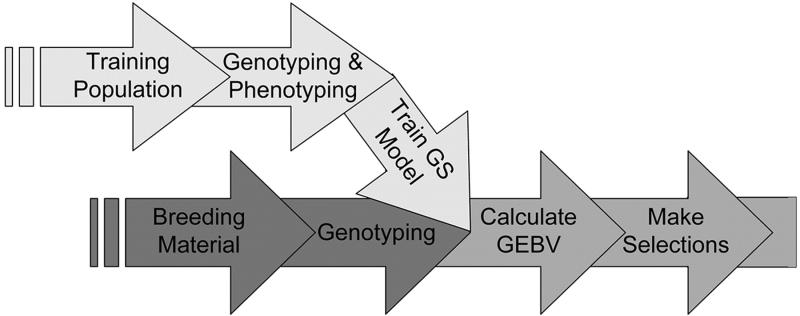
\includegraphics[width=0.49\linewidth]{figures/GS_process}
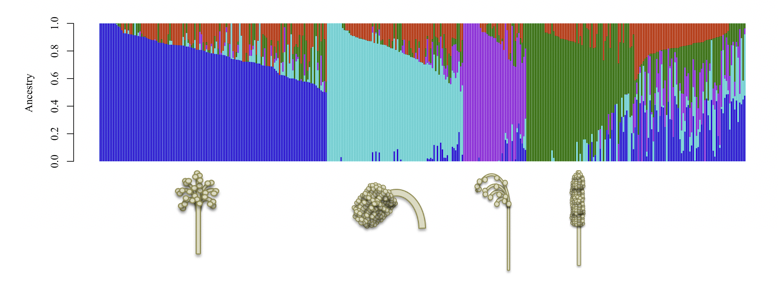
\includegraphics[trim={0 0.9cm 0 0},clip,width=0.49\linewidth]{figures/PopStr_SAP}
\captionof{figure}{\color{Green} Implementation of genomic selection model (\citep{heffner2009genomic}). Right: Population structure analysis of sorghum association panel (SAP). Each bar represents an individual and colors correspond to racial types caudatum, durra, guinea, kafir and mixed from left to right, respectively.}
\label{GS_pop}
\end{center}
\iffalse
While several studies have been conducted on genomic prediction for major crops like maize, wheat, soybean, etc., there are very limited empirical studies for GS in sorghum. Previous studies have shown that application of GS could help accelerate genetic gain in sorghum breeding programs \citep{hunt2018development,muleta2019optimizing}.\\
\fi
\smallskip
Our \textbf{OBJECTIVE} was to evaluate the effect of racial structure in genomic prediction for grain yield components in sorghum diversity panel (Fig. \ref{GS_pop}, right).\\

% \begin{center}
% \hspace*{\fill}
% 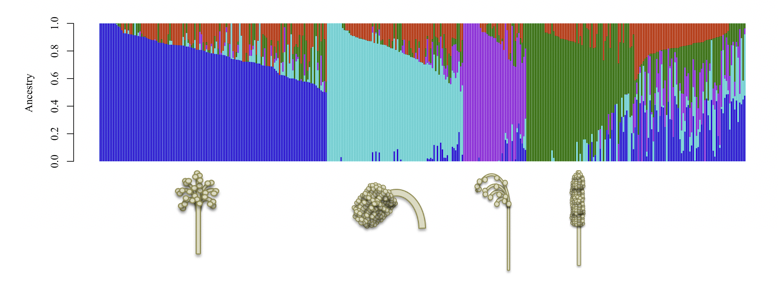
\includegraphics[trim={0 0.9cm 0 0},clip,width=\linewidth]{figures/PopStr_SAP}
% \captionof{figure}{\color{Green} Population structure analysis of sorghum association panel (SAP). Each bar represents an individual and colors correspond to racial types caudatum, durra, guinea, kafir and mixed from left to right, respectively.}
% \label{GS_pop}
% \end{center}

%----------------------------------------------------------------------------------------
%	METHODS
%---------------------------------------------------------------------------------------- 
\color{Black}
\fcolorbox{beige}{beige}{\parbox{0.495\textwidth \fboxrule}{%
\section*{DATA AND METHODS}
\begin{wrapfigure}{R}{0.33\textwidth}
%\begin{center}
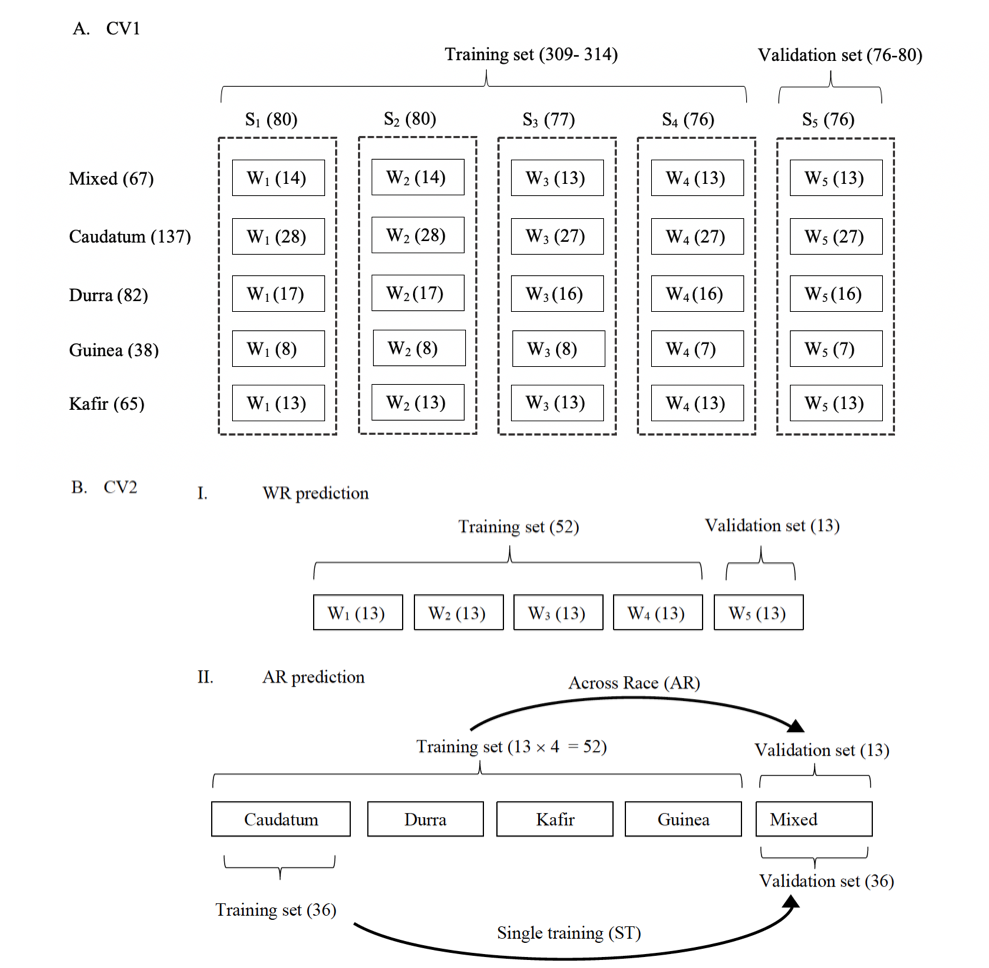
\includegraphics[width=\linewidth]{figures/CV_methods}
\captionof{figure}{\color{Green} Illustrations of cross validation methods.}
\label{CV_methods}
\end{wrapfigure}
%\end{center}
\hspace{0.1cm}$\bullet$ \textbf{Plant Material}: A total of 389 diverse accessions.\\
\hspace{0.1cm}$\bullet$ \textbf{Field Design}: RCBD with two replications, planted at PDREC, Florence, SC in 2013, 2014, and 2017 in two row plots.\\
\hspace{0.1cm}$\bullet$ \textbf{Prediction Model}: Genomic best linear unbiased prediction (GBLUP) using R package rrBLUP \citep{endelman2011ridge}:\\\\
\scalebox{1.5}{$ y_i = \mu + g_i + \epsilon $}\\\\
\hspace{0.1cm}$\bullet$ \textbf{Cross Validation (CV)}: Five-fold CV,\\
CV1 = stratified sampling,\\
CV2 = Across Race (AR), Within Race (WR), and Single Race Training (ST).\\ 
\hspace{0.1cm}$\bullet$ \textbf{CV1 Covariance decomposition}: R package MCMCglmm \citep{hadfield2010mcmc}:\\\\
\scalebox{1.2}{$Cov(x, y) = E_{race} [Cov(x, y|race)] + Cov_{race} [E(x|race), E(y|race)]$} \\%scalebox scales the texts into a desired size
}}

\vspace{-0.25cm}
%----------------------------------------------------------------------------------------
%	RESULTS
%---------------------------------------------------------------------------------------- 
\section*{RESULTS}

\fontsize{30}{25} \selectfont 
%\begin{wrapfigure}[30]{R}{0.2\textwidth}
\begin{center}
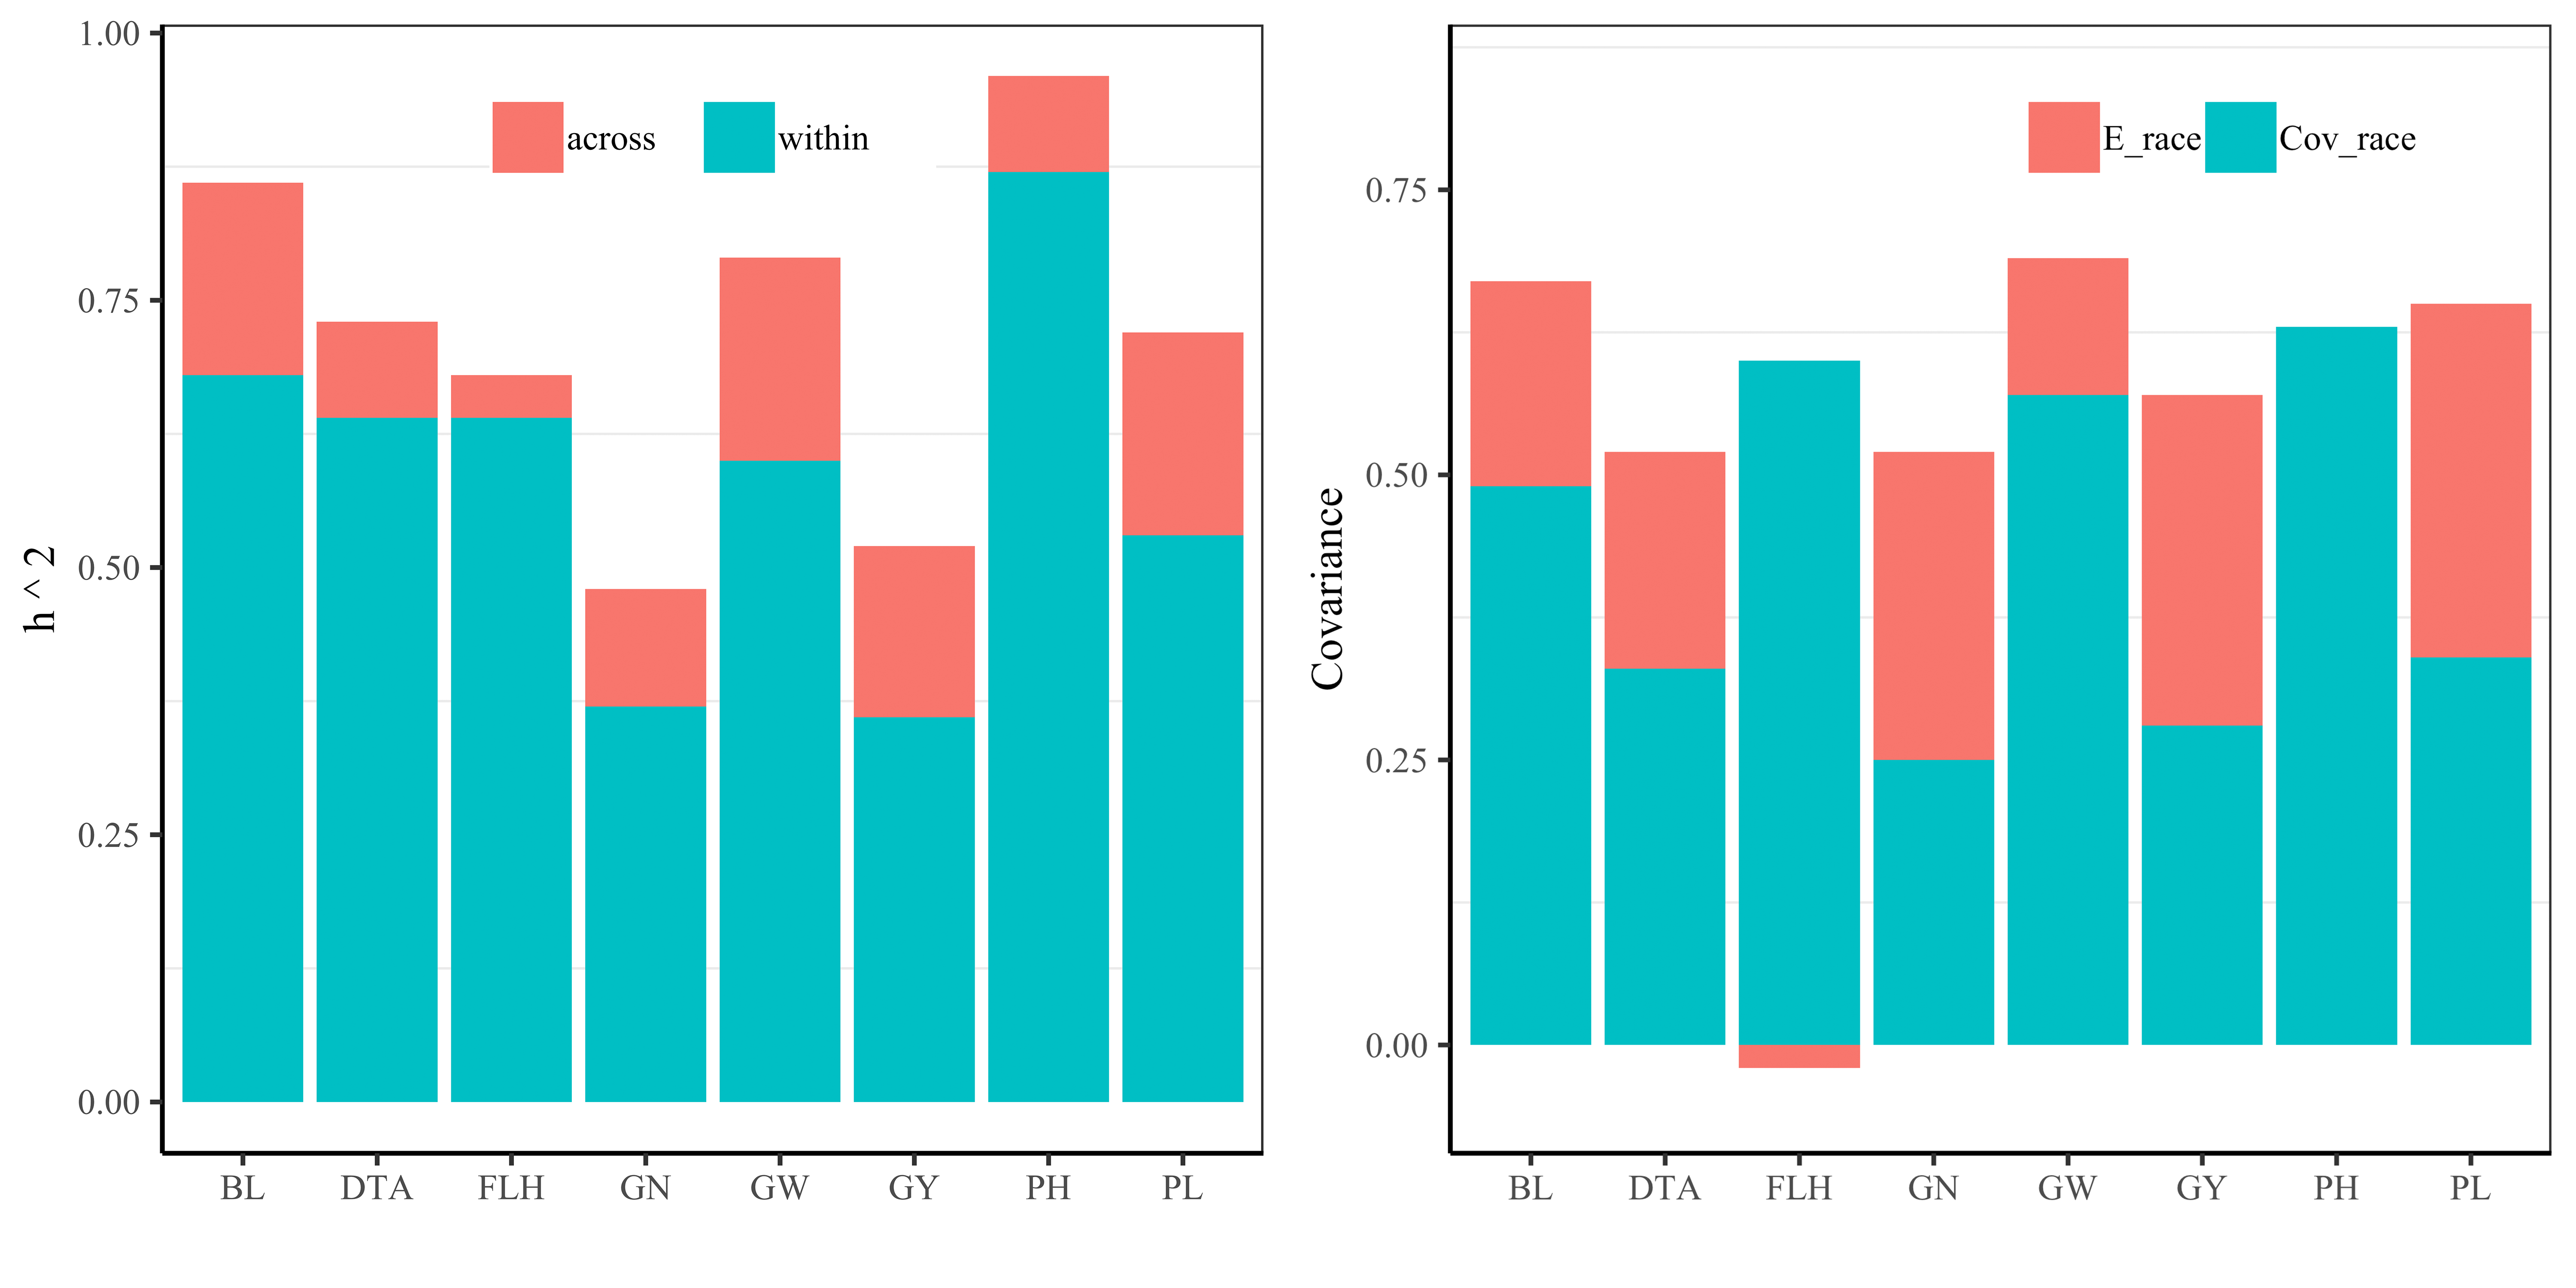
\includegraphics[width=0.45\textwidth]{figures/herit_Cov_CV1}
\captionof{figure}{\color{Green} Left: Within and across race genomic heritability. Right: Decomposition of covariances into expectation due to racial component (E\_race) and covariance due to individuals within a race (Cov\_race).}
\label{Covariance}
\end{center}
\smallskip
$\bullet$ Five clusters identified from population structure analysis, the clusters were broadly congruent with original racial classification (Fig. \ref{GS_pop}, right).\\\\
$\bullet$ Total genomic heritability was strongly correlated (\textit{r} = 0.6) to CV1 prediction accuracy across the traits.\\\\
$\bullet$ Although 80\% of total genetic variance could be ascribed to within group component, covariance due to race was larger than expected for panicle architecture and grain yield components (Fig. \ref{Covariance}).\\\\
$\bullet$ Mean \textit{r} in WR was greater than AR for races durra and caudatum, but little difference was seen for guinea, kafir and mixed.\\\\
$\bullet$ Although WR method had higher covariance estimates, relatively smaller difference in \textit{r} was seen due to larger variances in WR than AR.\\\\
$\bullet$ Mixed race had the highest \textit{r} as a training race whereas guinea had the highest \textit{r} as a validation race.
\newpage
%------------------------------------------
%\begin{wraptable}[13]{R}{0.23\textwidth}
\begin{center}
\captionof{table}{\label{tab1}\color{Green} Mean prediction accuracy for various cross validation methods. Values: mean $\pm$ standard deviation.}
\setlength{\tabcolsep}{15pt}
\begin{tabular}[width=0.9\textwidth]{ l  l  l  l  l }\\ \hline
Trait & CV1	& WR & AR & ST \\\hline
DTA	& $0.52\pm0.01$	& $0.24\pm0.23$	& $0.12\pm0.32$ & $0.11\pm0.23$\\
FLH	& $0.58\pm0.03$	& $0.41\pm0.23$	& $0.34\pm0.33$	& $0.32\pm0.21$\\
GN	& $0.52\pm0.02$	& $0.25\pm0.12$	& $0.27\pm0.30$	& $0.26\pm0.20$\\
GW	& $0.69\pm0.02$	& $0.61\pm0.10$	& $0.37\pm0.27$	& $0.43\pm0.20$\\
GY	& $0.57\pm0.02$	& $0.36\pm0.12$	& $0.35\pm0.30$	& $0.38\pm0.17$\\
PH	& $0.63\pm0.02$	& $0.46\pm0.15$	& $0.45\pm0.28$	& $0.36\pm0.18$\\
PL	& $0.65\pm0.01$	& $0.25\pm0.31$	& $0.12\pm0.33$	& $0.14\pm0.21$\\
BL	& $0.67\pm0.07$	& $0.38\pm0.24$	& $0.20\pm0.31$	& $0.26\pm0.19$\\\hline
\end{tabular}
%\end{wraptable}
\end{center}
\smallskip
%------------------------------------------
\begin{center}
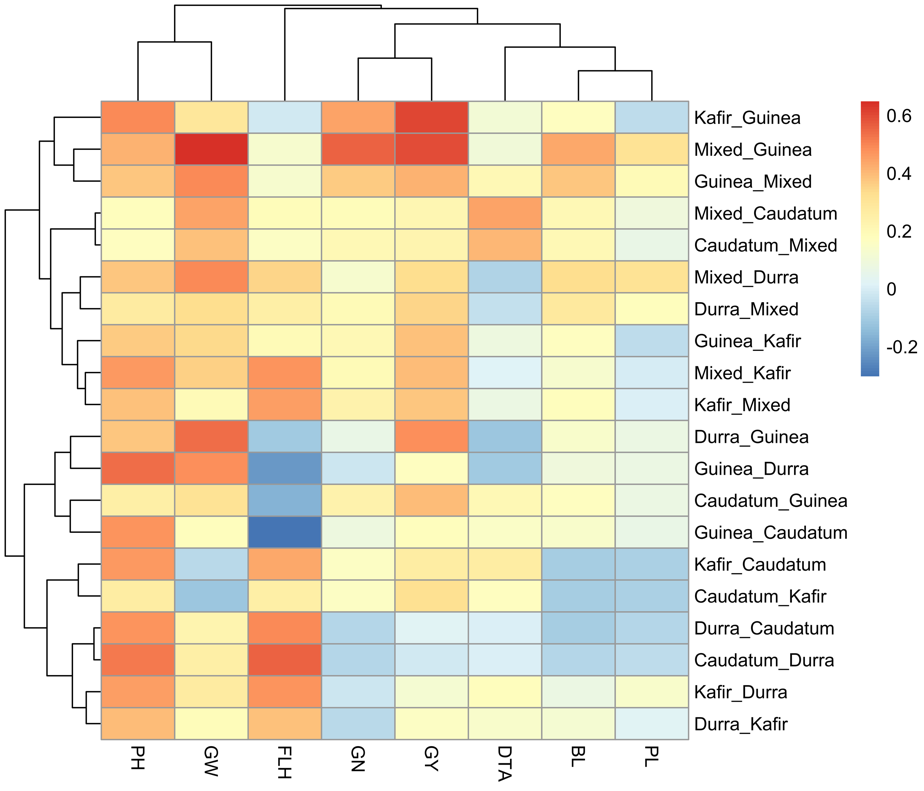
\includegraphics[width=\linewidth]{figures/SRT_accuracy}
\captionof{figure}{\color{Green} Heatmap and hierchical clustering of mean prediction accuracy by trait and prediction races' combination. Training and validation race for each combination is shown on the right of the heatmap, respectively.} 
\label{ST_TP}
\end{center}
\smallskip
% \begin{center}
% 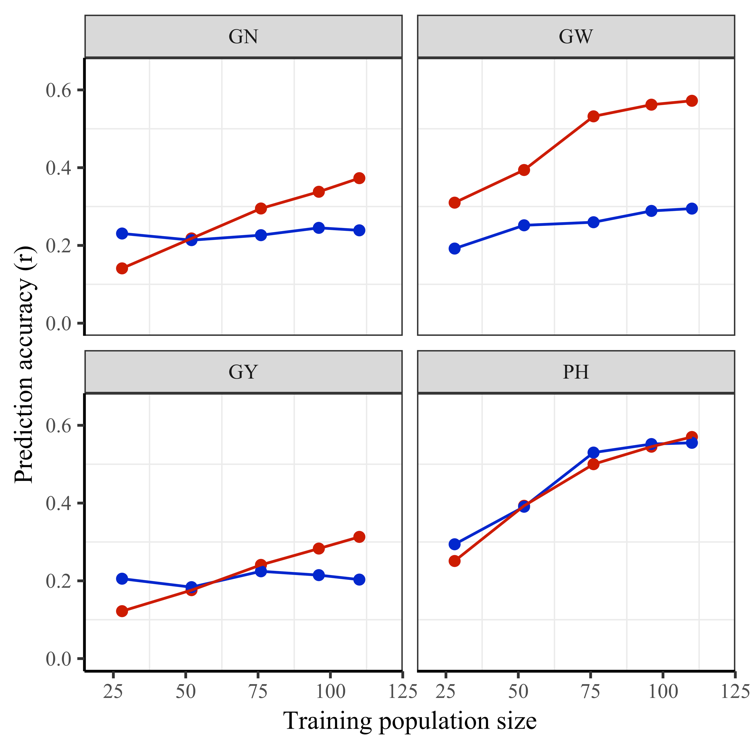
\includegraphics[width=0.4\linewidth]{figures/Caud_TPsize}
% \captionof{figure}{\color{Green}Left: Heatmap showing mean \textit{r} for combination of training \& validation races; trees show hierchical clustering for traits or prediction combinations. Right: Effect of training population size on WR (red) and AR (blue) prediction methods using caudatum as the validation race.} 
% \label{ST_TP}
% \end{center}
% \vspace{0.1cm}
%----------------------------------------------------------------------------------------
%	CONCLUSIONS
%----------------------------------------------------------------------------------------
\color{charcoal}
\fontsize{32}{25} \selectfont
\fcolorbox{bluebell}{aliceblue}{\parbox{0.49\textwidth \fboxrule}{%
\section*{SUMMARY}
% Our study highlights the importance of conducting empirical studies to test effect of population structure, genetic divergence, and genetic diversity in genomic prediction. The understandings can be crucial in designing a global diversity training population for germplasm characterization, screening, pre-breeding selection and population development. Here are the important highlights of our study:\\\\
\hspace{0.1cm}$\circ$ Prediction accuracy was boosted by the presence of similar population structure between training and testing population, as expected.\\\\
\hspace{0.1cm}$\circ$ Despite small between population genomic heritability, racial structure contributed a quarter to a half of CV1 covariances for panicle morphology and grain yield components. While higher than expected, this observation is not surprising because these traits are directly associated with sorghum racial classification. \\\\
\hspace{0.1cm}$\circ$ Genetic diversity in training population was as important as genomic relationship between training and validation race, especially for traits with complex genetic architecture and highly additive gene action. \\\\
\hspace{0.1cm}$\circ$ When evolutionarily younger races (caudatum and durra) with limited diversity and/or presence of private alleles were used as validation population, the genomic relationship outweighed the effect of genetic diversity.\\\\
\hspace{0.1cm}$\circ$ Based on our results, genomic selection in sorghum breeding programs with limited training size will largely benefit by adoption of genetically diverse training population with ancient and shared allelic variations.
}}
%----------------------------------------------------------------------------------------
%	REFERENCES
%----------------------------------------------------------------------------------------
\vspace{-0.5cm}
\color{Black}
\fontsize{20}{25} \selectfont 
\bibliography{bibliography}
\vspace{-0.5cm}
\section*{Abbreviations}
\fontsize{20}{25} \selectfont 
\textbf{AR} = across race, \textbf{BL} = terminal panicle branch length, \textbf{CV} = cross validation, \textbf{DTA} = days to anthesis, \textbf{FLH} = flag leaf height, \textbf{GN} = grain number, \textbf{GW} = grain weight, \textbf{GY} = grain yield, \textbf{PH} = plant height, \textbf{\textit{r}} = correlation/prediction accuracy, \textbf{SNP} = single nucleotide polymorphism, \textbf{ST} = single race training, \textbf{WR} = within race.
%----------------------------------------------------------------------------------------
%	ACKNOWLEDGEMENTS
%----------------------------------------------------------------------------------------
\vspace{-0.5cm}
\section*{Acknowledgment}
\vspace{-0.5cm}
\begin{center}

\includegraphics[trim={0 1cm 0 1cm},clip,width=\linewidth]{figures/funding_sources2}
\end{center}
\end{multicols}
%\textcolor{NavyBlue}{\rule{\linewidth}{15pt}}
\vspace{-0.5cm}
\end{framed}
\end{minipage}
%\hspace*{0.1cm}
\end{document}
%----------------------------------------------------------------------------------------
%%%%%%%%%%%%%%%%%%%%%%%%%%%%%%%%%%%%%%%%%%%%%%%%%%